
\chapter{The Steganos Project}
\begin{multicols}{2}
Steganos is the name of the application that implements the algorithms enumerated in the earlier chapters of this paper and is the direct result of the work done by the authors. In this chapter I will present what modern technologies and frameworks went into creating the application, how it is structured from an Object Oriented point of view, how fast it is and how I hope it will expand into the future.

\section{Used technologies}
\subsection{C++}
C++ is one of the lowest high-level computer programming languages. Designed by Bjarne Stroustrup, it first appeared in 1985 as a variation of one of the most popular languages at the time, C. It is one of the most efficient modern languages mainly because it has been designed with performance and flexibility in mind, just like its predecessor. C++ has gained a lot of traction  from big companies like Intel and Microsoft which needed a programming language that could be used for operations ranging from basic kernel functions to highly specialized Object-Oriented projects with Graphical User Interfaces\cite{stroustrup_2018}.

Since its conception, C++ has grew substantially by adding support for generic and functional features to ease the development processes and getting standardized by the International Organization for Standardization probably helped as well because it meant no more obscure variations of the language, allowing programmers to follow only one standard, ending up with even more portability and stability of the applications.

In the modern day, it is used almost everywhere: the kernel of various operating systems, the transaction software used by banks, drones and airplanes, embedded systems such as the Arduino or Raspberry Pi, and now in the Steganos Project as well under the latest approved standard of the language, C++17.

C++ inherited from C the file types: headers and sources. The header files (the files that have a .h or .hpp extension) are where the standard recommends to store the class declarations, function prototypes, constants declarations, no definitions should take place in a header file. There are a few exceptions to this rule, the most common one being a rule that states that all templated functions and functions are to be declared and defined in a header file otherwise it will not work properly when dealing with multiple instances of different types. In the case of the source files (the files that have the .c or .cpp extension) the standard suggests to only be used for the definition of the class methods or other general functions. Following the standard results most of the time in a clean and well defined separation in the code, allowing for high cohesion and low coupling in all projects built using C++.

The reason for choosing C++ as the language for the Steganos project is simple: it allows for the programmer to work on the raw bytes of files in an extremely easy way, reading and parsing them, bit-wise operations and writing to file, all the common low-level operations that are highly valued when working in the steganography field. But the high level aspects of the language also permit for dealing with complex tasks, such as modern cryptography algorithms applied to robust byte streams or holding all the information in different data structures.

\subsection{CMake}
CMake is a cross-platform open-source tool designed for managing the build process of software based on the C++ programming language. It has been created in the year 2000 and ever since then it stayed compiler-independent using simple configuration files that generate the adequate makefiles to be used in the users environment while building the target project\cite{cmake}.

CMake uses files called CMakeLists.txt that contain the commands to be used by the internals of the tool in the building process. It is required that one file is in the root of the project before running the CMake process, with the possibility of adding a .txt file in the subdirectories in order to indicate special cases that require a different approach.

\begin{figure}[H]
    \centering
    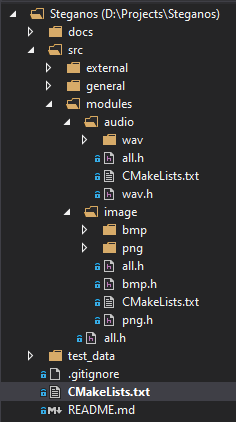
\includegraphics[height=6.9cm,keepaspectratio]{pics/cmake_folder_structure_example}
    \caption{Folder structure of a project using CMake}
\end{figure}

Each command in CMake has the same format: COMMAND (args..). Using this format, users are able to build even the most complex software projects in the form of simple executables, dynamic or static linked libraries, etc. Steganos uses CMake because it is an extremely effective tool in the building process and it allows for separating the logic of the project into distinct modules i.e. the audio module, the image module, the general usage module, and linking them in the end into a simple executable. Most projects use only a small subset of the commands available in CMake, the most common being:

\begin{itemize}
  \item \textbf{CMAKE\_MINIMUM\_REQUIRED} is used to mark the minimum version of CMake that is required to be installed on a system in order to build the project.
  \item \textbf{SET} is used to assign a value to a CMake variable that is used while building, similar to environment variables found on all operating systems.
  \item \textbf{PROJECT} for naming the project, important step in active Continous Integration and Continous Development environments.
  \item \textbf{INCLUDE\_DIRECTORIES} for marking the directories containing the header files in order for the compiler to be able to link the source files and header files.
  \item \textbf{ADD\_EXECUTABLE} for creating an executable after build the project from the source files given as arguments.
  \item \textbf{ADD\_LIBRARY} for creating a library or module with the given source files.
  \item \textbf{TARGET\_LINK\_LIBRARIES} for linking (pre)defined modules or executables between eachother.
\end{itemize}


\subsection{CXXOpts}
CXXOpts is an open-source C++ library that is meant to be a lightweight command line option parser\cite{jarro2783_2020}. It is meant as the C++11 and beyond alternative to other libraries such as Commons CLI for Java or Argparse for Python. It was initially created by user jarro2783 on Github and nowadays is actively developed by the community using the Git commit and pull request system. CXXOpts is made to replicate the handling of the help argument and the merging of multiple parameters commonly found in *NIX command line binaries, without using any additional dependencies in a header-only file.


\subsection{Lodepng}
Lodepng is an open source C++ library developed by Lode Vandevenne used for image processing for pictures stored under the PNG format \cite{lvandeve_2020}. It is very useful for decoding the image data before beginning the steganography process, making it easy to modify the data and to encode it back into a PNG file that follows the standard format. Lodepng works on every version of C++, contains only two files(a source file and a header file) and is rated to be one of the fastest libraries for PNG image processing. Steganos uses Lodepng to parse PNG files and to obtain the image data byte stream from the zlib compressed stream in order to be able to work with the implemented steganographic algorithms.

\subsection{Robot36 SSTV Engine}
Robot36 is a library created by Ahmet Inan in order to be able to encode and decode images using the Slow Scan Television (also known as SSTV) format, more specifically the Robot36 standard. The library is open-source and is available on github\cite{robot36_git}. By default it supports only color BMP images that are 320 pixels wide and 240 pixels tall and can be compiled using any C compilers only under a Linux system which has the Advanced Linux Sound Architecture (ALSA) libraries installed. Since Steganos is a C++ project that the authors intended to be cross-platform, we have forked the original project and refactorized the code to be buildable and to work on the Windows architecture as well. After some more refactorization is done, we have every intention to release our version of the SSTV Engine and to create a pull request to the original repository.

\begin{figure}[H]
    \centering
    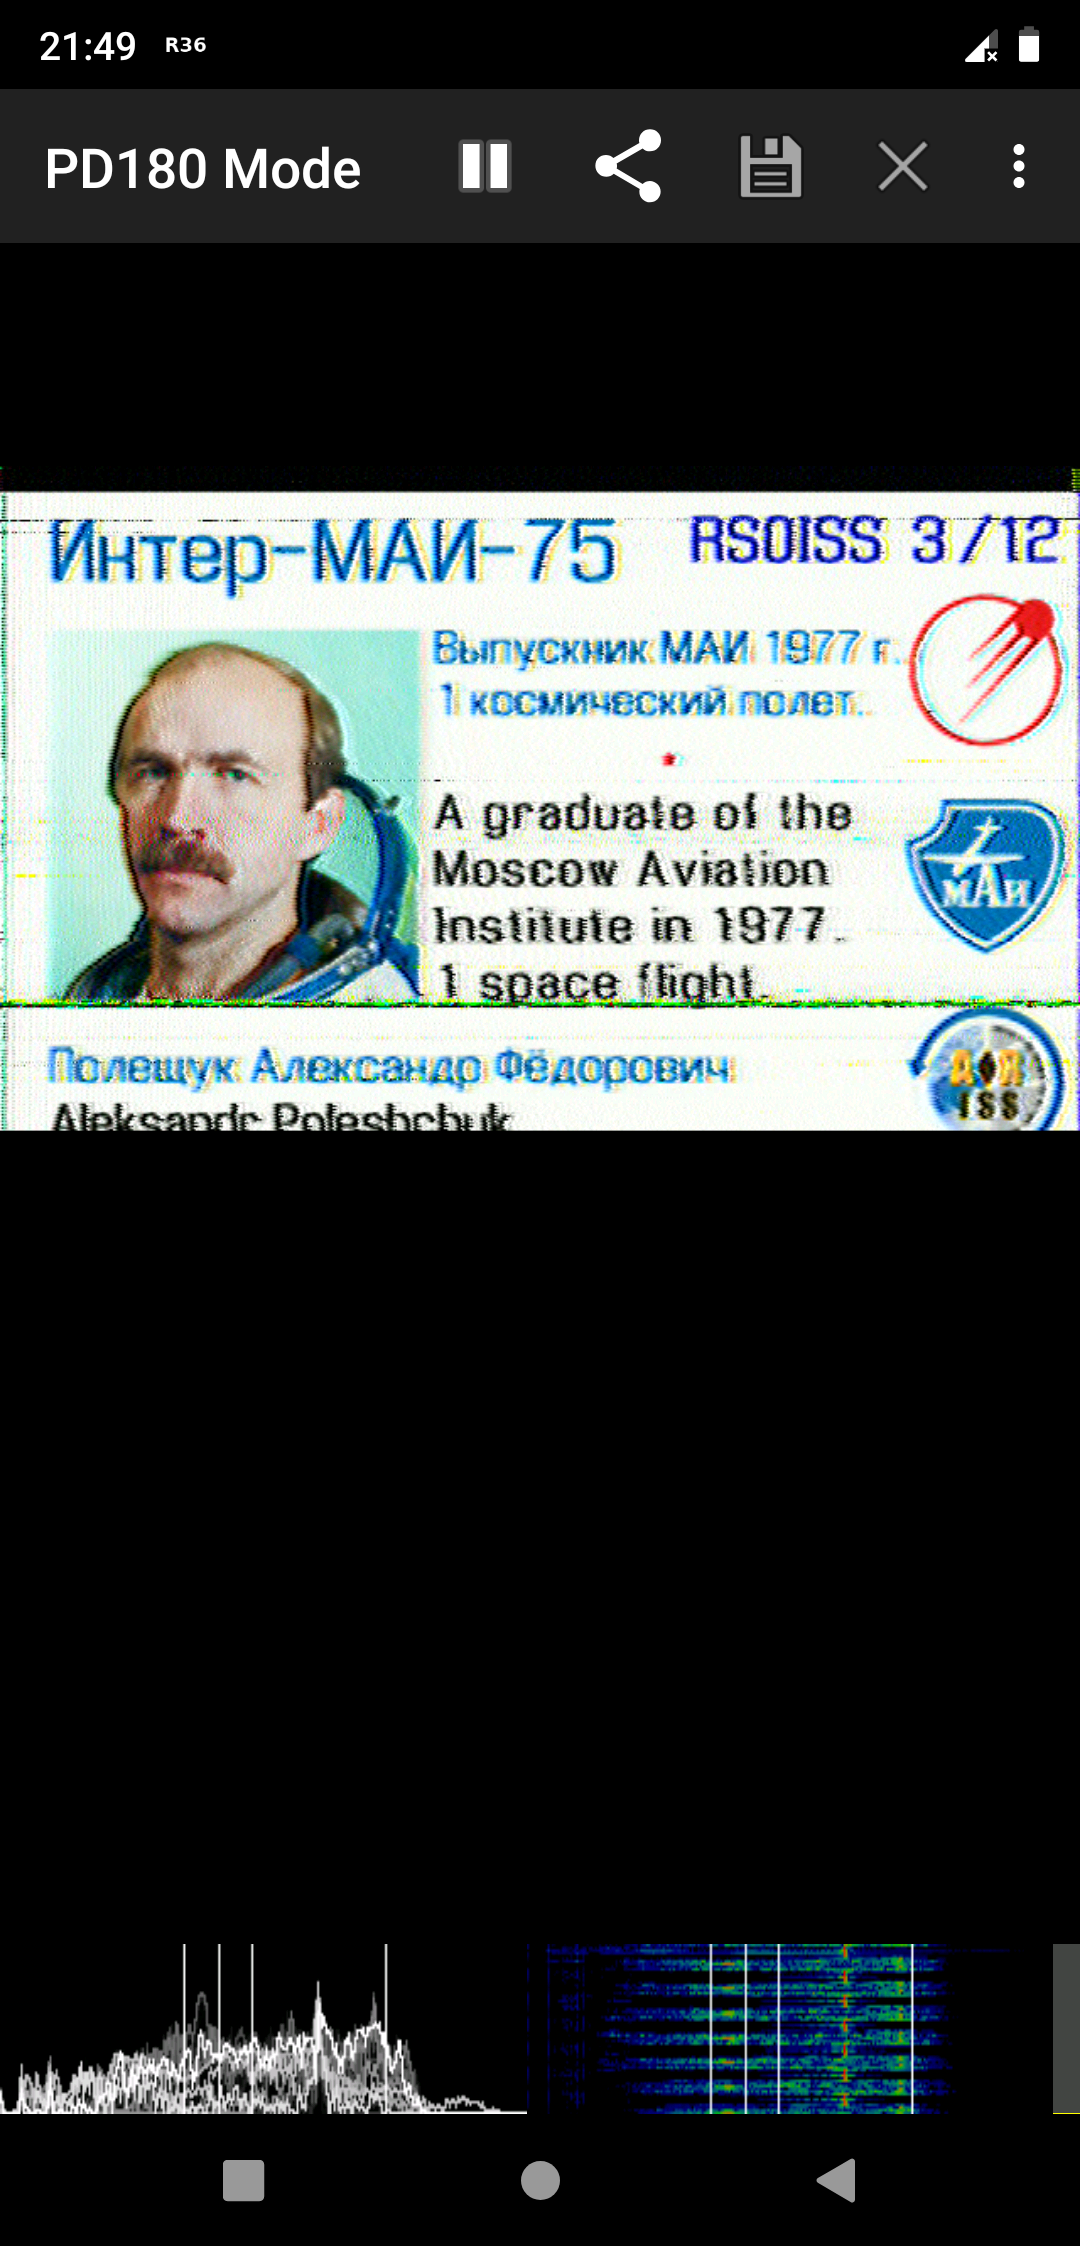
\includegraphics[height=7.5cm,keepaspectratio]{pics/application_chapter/sstv_example_iss}
    \caption{SSTV Engine decoding transmission from the International Space Station}
\end{figure}

\subsection{Jenkins}
Jenkins is one of the biggest open source automation servers that is meant to automate the process of building, deploying, testing etc. any project. Developed in Java, it supports a big range of popular languages and frameworks, either by default configuration or by installing a plugin available on their developer page. We picked Jenkins for Steganos due to previous working experience of the authors with it and since it has the ability to build and release C++ and CMake projects using a single plugin it has proven to be an extremely valuable asset in maintaning a continuous integration and continuous delivery schedule of the project.

\begin{figure}[H]
    \centering
    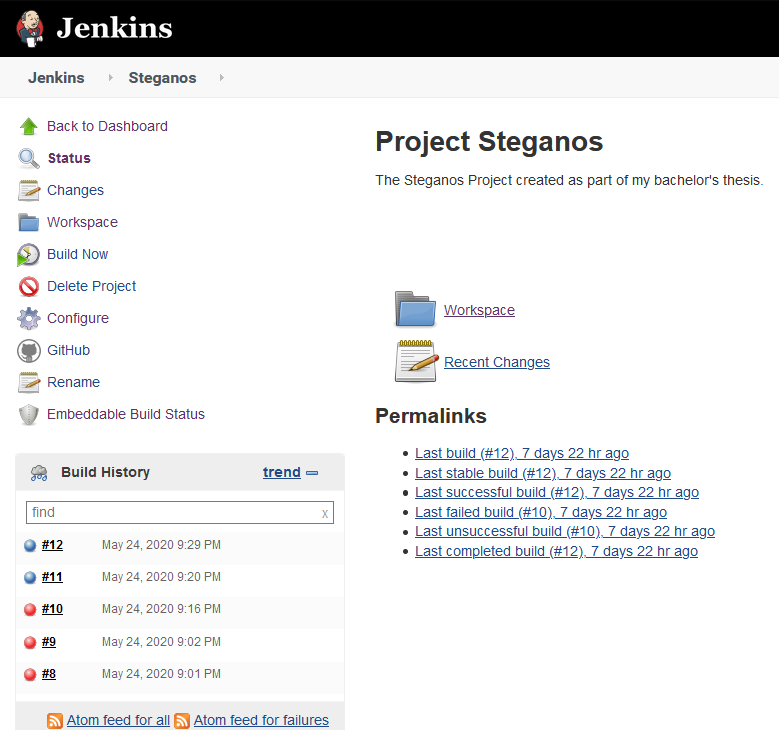
\includegraphics[height=7.5cm,keepaspectratio]{pics/application_chapter/steganos_jenkins_job}
    \caption{Jenkins management interface of the Steganos job}
\end{figure}


\section{Application architecture}
The Steganos Project is an application that uses the Object Oriented Programming aspects in order to achieve the best performance while maintaining high cohesion and low coupling between the components of the codebase. The project is structured in multiple modules\footnote{To be technically correct they are only different folders because the latest available C++ standard as of the time of writing this thesis is C++17 which does not understand yet the concept of modules. However developers should rejoice over the announcement made by Microsoft to standardize C++ modules starting with the C++20 standard\cite{N4720}.} that were built to be as independent as possible with the goal to provide steganography functions for the supported file formats. The main module contains the source files for the entry point of the application which processes the arguments given via the command line along with the code for some of the utilities, helper function that help convert pixels between different representations(YUV, RGB, BGR, YCbCr) or bit-wise operations such as toggling the last significant bit or building a byte using the LSBs from a byte stream. The algorithm module declares and defines the algorithms that are implemented in the application, all of which have been discussed thoroughly in the earlier chapters of the thesis (LSB insertion, embedding secrets into file metadata, use-after-end encoding). The remaining modules all follow the same design patterns and are responsible for the parsing of the cover files and the encoding or decoding of hidden digital files inside them. 

We can see in figure \ref{module_overview} the overview of the entire application and what each module contains more specifically. This is only a very simplistic rendering of the module deployment, we will delve in for a more in-depth perspective later this chapter.
\end{multicols}

\begin{figure}[H]
    \centering
    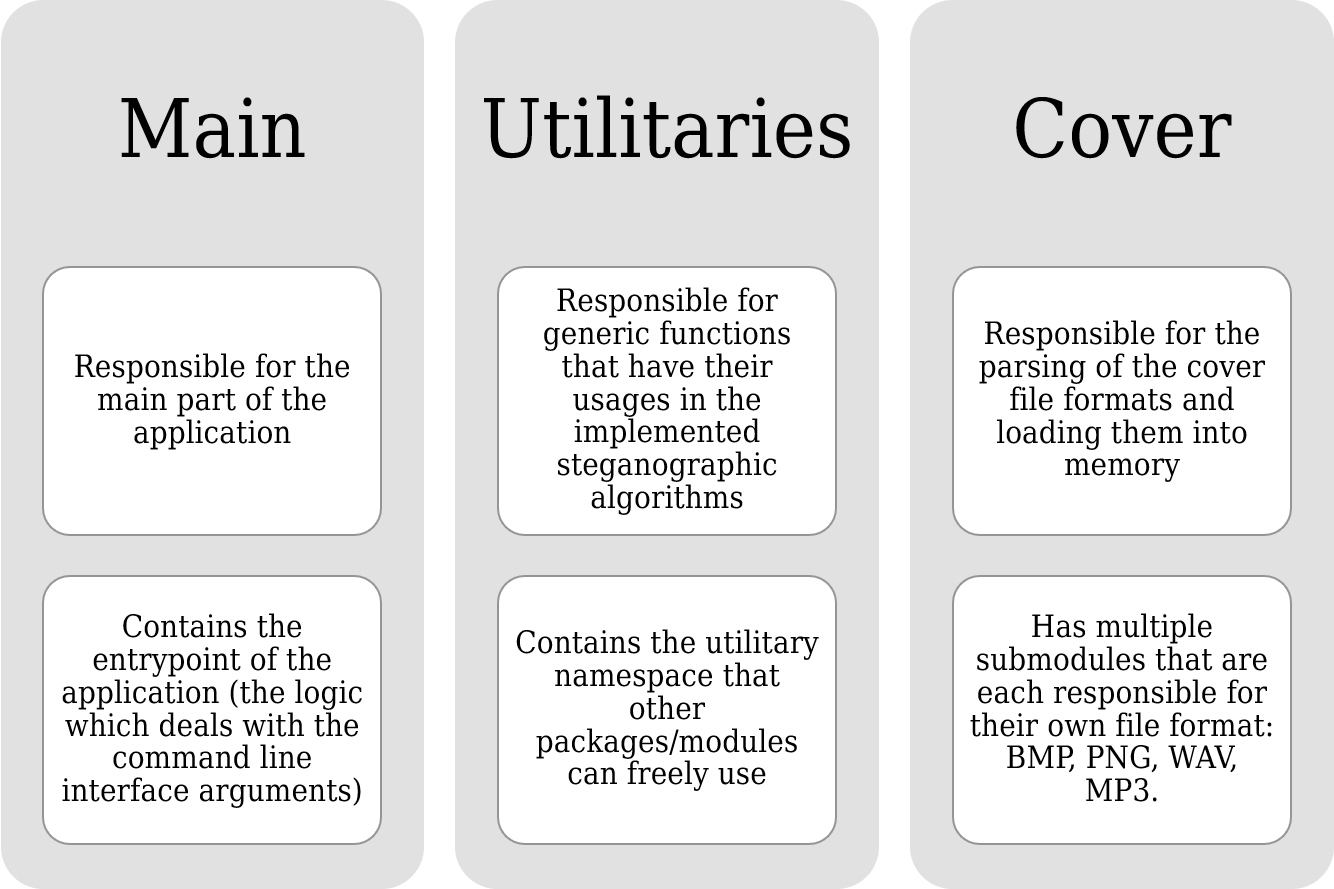
\includegraphics[width=13cm,keepaspectratio]{pics/application_chapter/module_overview}
    \caption{Overview of the Steganos modules}
    \label{module_overview}
\end{figure}

\begin{multicols}{2}
In figure \ref{cover_module_overview} we can see a class diagram of the general struture of each of the four aforementioned cover submodules (the codebase which deals with parsing the cover files that allow for the steganography algorithms to have the necessary data to work with). 
\end{multicols}
\begin{figure}[H]
    \centering
    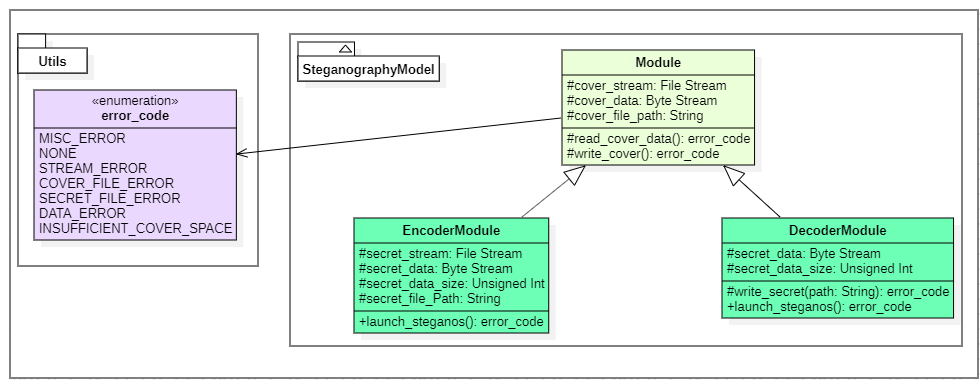
\includegraphics[width=16cm,keepaspectratio]{pics/application_chapter/diagrama_module_interface}
    \caption{Structure of a cover module}
    \label{cover_module_overview}
\end{figure}

\begin{multicols}{2}
After seeing how the project is structured into modules and submodules, what classes, interfaces, methods and attributes we have, it is also very important to understand how the data flows from the moment we launch Steganos to the moment the output file is generated (the output file is either the cover file containing a secret message, either the actual secret message, depending on the option used). In figure \ref{flowchart-code} we can see a flowchart of the application containing the key points of the entire process.
\end{multicols}
\begin{figure}[H]
    \centering
    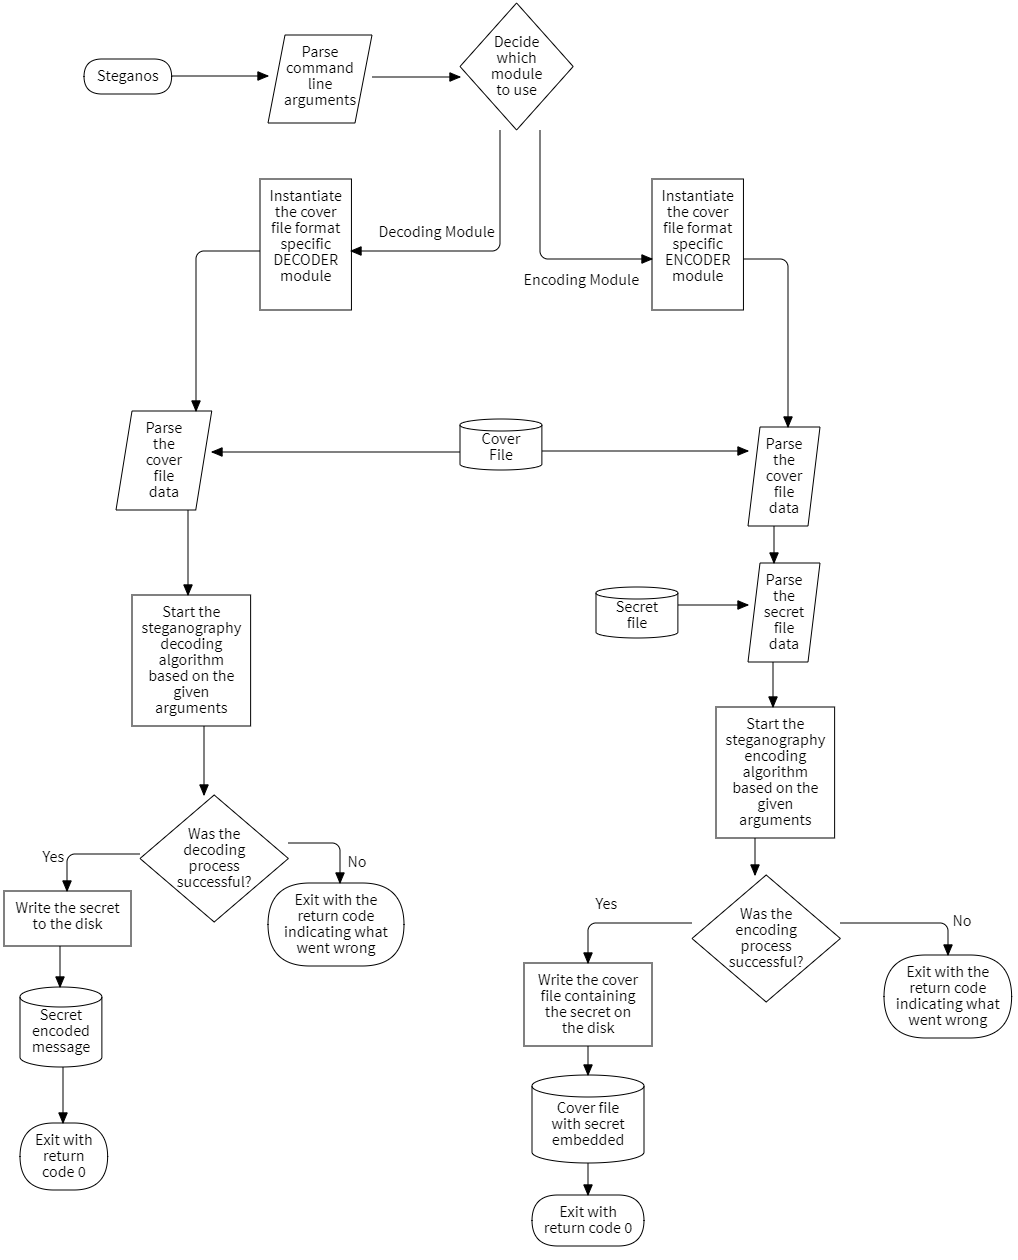
\includegraphics[width=15cm,keepaspectratio]{pics/application_chapter/flowchart}
    \caption{Steganos code flowchart}
    \label{flowchart-code}
\end{figure}

\begin{multicols}{2}
To make sure that the project will always be in at least a buildable state after any commit is done we are using Jenkins. It is very important to make sure that the code compiles and that if there are any errors, the authors are aware of them and will have the option to hold back the release until the issues are fixed. On a more related note to the Steganos application, we have the following job configuration for testing each new version before releasing:
\begin{itemize}
	\item Maximum number of build to keep is set to 5 to conserve total storage used.
	\item Each new commit on the master branch will activate the hook trigger to let Jenkins know that a new version is available and that it should try to build it.
	\item Using the "Unix Makefiles" generator to set up the CMake build files with the build type set to "Release".
	\item Publish the build result to the project page to keep it up to date to the current release or trigger custom personal alerts to notify in case of failure.
\end{itemize}
\end{multicols}

\begin{figure}[H]
    \centering
    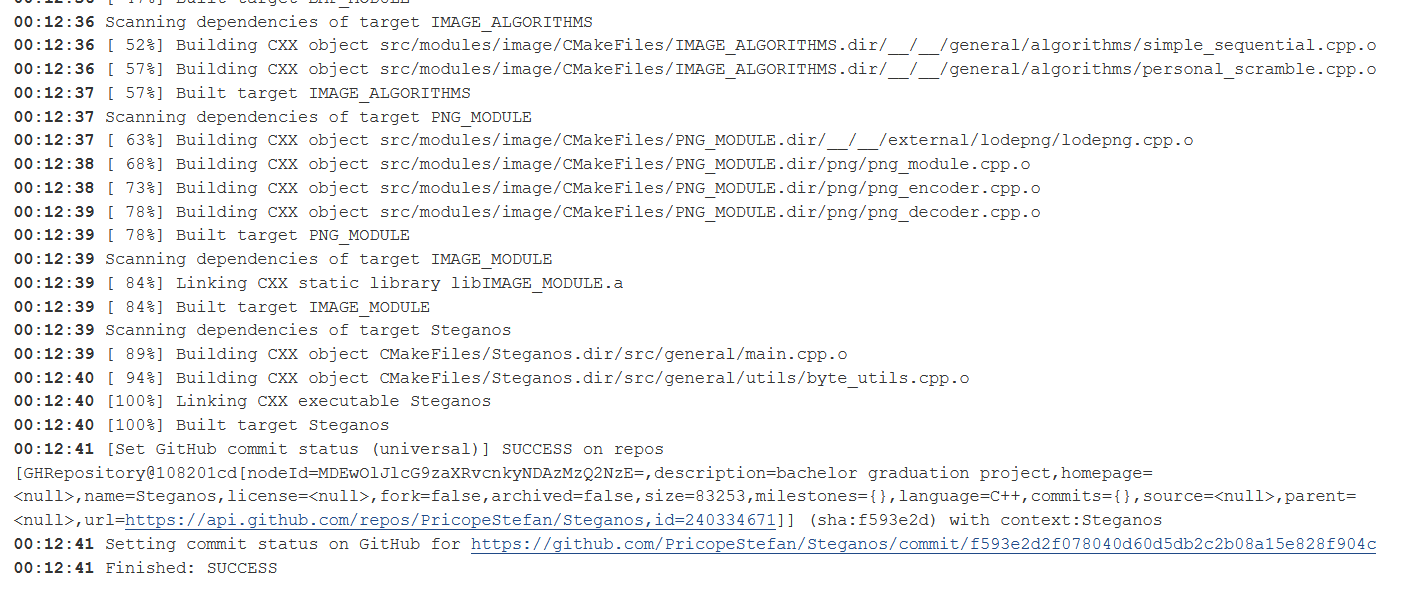
\includegraphics[width=15cm,keepaspectratio]{pics/application_chapter/jenkins_project_build}
    \caption{Jenkins log of the Steganos job build}
    \label{jenkins-log}
\end{figure}


\definecolor{dkgreen}{rgb}{0,0.6,0}
\definecolor{gray}{rgb}{0.5,0.5,0.5}
\definecolor{mauve}{rgb}{0.58,0,0.82}
\lstset{frame=tb, %configurare listing format pt subcapitolul asta
  language=C++,
  aboveskip=3mm,
  belowskip=3mm,
  showstringspaces=false,
  columns=flexible,
  basicstyle={\small\ttfamily},
  numbers=none,
  numberstyle=\tiny\color{gray},
  keywordstyle=\color{blue},
  commentstyle=\color{dkgreen},
  stringstyle=\color{mauve},
  breaklines=true,
  breakatwhitespace=true,
  tabsize=3
}

\begin{multicols}{2}
\section{Implementation details}
Steganos contains many critical parts that are required to succeed in order to work properly. If any part of code or function call were to fail we would need to know so that we can properly interrupt the process on our terms, free any dynamically allocated memory, log the error messages so that developers are aware of any bugs that may appear or if the application is in a release form, notify the client of what has happened and why the application failed. Since C/C++ is a rather monstrous amalgamation when talking about exceptions raised during runtime execution (at least in the standard libraries, more complex frameworks like Boost do not suffer as much from this), we have preferred to validate the function calls based on a more simple method, the code returned by the function which is basically a glorified integer that has some meaning attached to its values. You can see in listing \ref{lst:try_macro} the exact define macro used in the project and in listing \ref{lst:try_macro_example} an example from one of the encoder module constructors.

\end{multicols}
\begin{lstlisting}[language=C++, caption=The TRY macro used for any critical operation,label={lst:try_macro}]
 #define TRY(X) generic_assert((X), __FILE__, __LINE__);
 inline void generic_assert(error_code code, const char* file, int line) {
   if (code != error_code::NONE) {
     printf("[Assert error]Message = %d in file %s at line %d\n", code, file, line);
     exit(static_cast<int>(code));
   }
 }
\end{lstlisting}

\begin{lstlisting}[language=C++, caption=Usage example of the TRY macro,label={lst:try_macro_example}]
WAVEncoderModule::WAVEncoderModule(const char* cover_file_path, const char* secret_file_path) : WAVModule(cover_file_path) 
{
  TRY(utils::load_stream(secret_file_path, secret_stream));
  TRY(utils::read_byte_stream(secret_stream, secret_data, secret_data_size));
}
\end{lstlisting}


\begin{multicols}{2}
\section{Using the application}
Steganos was designed to be a very simple command line tool that is fast, reliable and portable. Using Cxxopts we have tried to implement an intuitive way of passing the arguments to the program, such that they all make sense and that any of the available configurations and command executions are easy to understand. You can see from the program output below that it is very easy to learn the options available to the end user by adding the -h flag and see what is supported and what not.
\end{multicols}
\begin{verbatim}
D:\Projects\Steganos\out\build\x64-Debug>Steganos.exe
You must specify one cover file.
Do Steganos.exe -h for more information.

D:\Projects\Steganos\out\build\x64-Debug>Steganos.exe -h
Simple steganography project created as a part of my bachelor's thesis
Usage:
  Steganos [OPTION...]

 Encoding/Decoding options:
  -c, --cover FILE   The file that serves as a cover for the secret message
  -s, --secret FILE  The secret file which will be embedded into the cover
                     file - ENCODING ONLY

 General options:
  -o, --output FILE             Name of the output file (default: output)
  -v, --verbose                 Verbose output
  -m, --method METHOD           The method to be used when encoding/decoding
                                the message
  -p, --passkey PASSKEY         The password used to secure the message or to
                                decipher it (default: password)
  -h, --help                    Prints this help message
\end{verbatim}

\begin{multicols}{2}
Based on the information above, it is almost trivial to come up with working command examples based on the help menu we displayed earlier. We can begin looking at some examples to see how Steganos works. Let's assume that we want to encode a secret message stored in a txt file within a BMP file. All we would need to type is the path to the secret file and the path to the cover file. The output can be seen below.
\end{multicols}
\begin{verbatim}
D:\Projects\Steganos\out\build\x64-Debug>Steganos.exe --cover marbles.bmp --secret secret.txt
Done
\end{verbatim}

\begin{multicols}{2}
That's all there is to it. However to some the need to type so many characters without any autocomplete (because option autocomplete is not commonly available in most shells) could be an annoyance so Steganos also offers the option for shortened option names to make the process quicker.
\end{multicols}
\begin{verbatim}
D:\Projects\Steganos\out\build\x64-Debug>Steganos.exe -c marbles.bmp -s secret.txt
Done
\end{verbatim}

\begin{multicols}{2}
We also have the option to enable verbose output to see debugging information in real time during the Steganos process and see exactly what it is doing. We can also specify the name of the output file to be whatever we would like it to be.
\end{multicols}
\begin{verbatim}
D:\Projects\Steganos\out\build\x64-Debug>Steganos.exe -c marbles.bmp -s secret.txt 
                                      \\ -o super_secret_marbles.bmp -v
BMP Image data is found beginning at 54
Ignoring 0 bytes to get to the actual image data
Available methods:
SEQUENTIAL (default)
PERSONAL_SCRAMBLE
No encoding method specified! Picking default option.
Deleted image data and its associated stream
Done
\end{verbatim}

\begin{multicols}{2}
\section{Further work}
Regarding the future of Steganos, I hope that it will be fairly fruitful and worthwhile. The entirety of this thesis we have only laid down the groundwork of the project and have talked about the most basic and essential part of the application. However, the possibilities for extending Steganos are almost endless and during the time while building the application and writing this thesis I have saved some of the more note-worthy ideas that came to my mind (in no particular order):
\begin{itemize}
	\item \textbf{Additional file formats support}. Right now Steganos only supports 4 major file formats, two digital image formats (BMP and PNG) and two audio formats (WAV and MP3). However, there are a lot more file formats that are commonly used on the Internet and that could be viable picks as a cover in the steganography process. Some of those formats include but are not limited to: Joint Photographic Experts Group (JPEG images) format, Free Lossless Audio Codec files (high-quality audio files, commonly found on album disks), Graphic Interchange Format (GIFs) and many more. 
	\item \textbf{Proxy server and chat application}. This is one of best development Steganos could get in my opinion. As mentioned earlier, right now the project is similar to only a core-engine library that just takes some input, processes it and turns it into an output. It is not integrated anywhere, it's just a simple CLI application. However, it would be nice to see it integrated into a chat application, following a very simple idea: run Steganos as a server process which accepts any kind of message and returns a multimedia file that has the secret embedded within and then send that image/audio/video file to the peers. They would be able to decode the message based on an already negociated process (the negociation took over a secure channel that any intruders would not have access to) and they would be able to reply in the same manner. The clients could also change the encoding/decoding process automatically and then notify the peers by also embedding the renegociation in the cover file. This application has the advantage that it only needs a brief secure environment for the initial connection and then be able to securely coomunicate over any type of channel. It would certainly be one of the most interesting usages for a steganography project, mostly because it would be practical enough to be used in real world situations and not just Capture the Flag challenges.
	\item \textbf{Windows integration for Jenkins}. At the moment of writing this, there is only one deployed instance of Jenkins running the Steganos job and it is based on Linux. That means that the only types of files that are automatically generated and tested are only the Linux binaries since there is no easy way of also building the Windows binaries. Some research has revealed that there is the option of adding a Windows based Jenkins instance in a master-slave configuration that would technically allow the full building and testing of the executables but we have not yet managed to implement this. 
	\item \textbf{Additional algorithms}. Most algorithms described in this paper are implemented in the Steganos project but there are plenty viable ones (especially those that rely on scrambling the data) that have not seen yet the light of day. It would certainly be interesting to add them and compare them to existent implementations or to the other methods.
	\item \textbf{Encrypting the secret}. Even though the option is specified in the help menu, it is not yet possible to encrypt the actual secret, mainly because I could not decide on which encryption methods to make available and because I also would rather focus on building the core codebase and to implement the steganography algorithms first. However, it is almost mandatory that the option of encrypting the secret before the embedding process is added in a future release to increase the security of the contents.
\end{itemize}
\end{multicols}